\chapter{Explainable Artificial Intelligence Results}
\label{chap:xai_results}

\section{Chapter Overview}

This chapter presents the outputs produced by the standardised \gls{xai} framework for the five final analytical configurations. The evaluation extends beyond reporting feature rankings. It examines agreement among global explanation methods, persistence of rankings across repeated fits, local explanations of correct and erroneous predictions, recurring patterns across datasets and model families, and the capabilities demonstrated by the framework. These dimensions reflect the broader view that \gls{xai} methods should be evaluated according to properties such as agreement, stability, and suitability for the analytical task \citep{mohseni_multidisciplinary_2021, vilone_classification_2021, lofstrom_meta_2022, canha_functionally-grounded_2025}.

The results were generated from the evaluated configurations described in Chapter~\ref{chap:validation_results}. Native importance, permutation importance, and mean absolute \gls{shap} values quantify different aspects of model behaviour and have different numerical scales \citep{fisher_models_2019, NIPS2017_8a20a862, linardatos_explainable_2020}. Their raw magnitudes are therefore interpreted only within the corresponding method and dataset. Comparisons among methods use feature ranks and top-five membership. The local analysis uses the presence of feature names in \gls{lime} rules and the signed weights assigned by the local surrogate. \gls{lime} weights are not treated as directly comparable with global importance magnitudes \citep{ribeiro_why_2016, vilone_classification_2021}.

For Heart, Stroke, Diabetes, and \gls{ckd}, the explanations describe models evaluated using held-out test observations. \gls{hbaone} instead provides in-sample explanations of a full-cohort inferential model whose encoded design matrix contains both main effects and interaction terms \citep{strack_impact_2014}. Its explanation results are therefore interpreted separately from the four held-out predictive configurations.

Together, these analyses assess whether different explanation methods emphasise the same features, whether global rankings remain stable across bootstrap refits, whether correct and erroneous predictions share similar local rules, and whether the framework produces consistent analytical outputs across heterogeneous configurations. The chapter therefore evaluates explanation behaviour and framework coverage in addition to reporting substantive feature rankings.

\section{Global \gls{xai} Results by Dataset}

Each combined importance plot displays five entries. For Heart, Stroke, Diabetes, and \gls{ckd}, these entries represent model features. For \gls{hbaone}, they represent encoded design-matrix terms, including categorical contrasts and interactions. Within each dataset, the values from each explanation method were divided by the maximum value produced by that method. The five displayed entries were then selected according to their mean normalised importance across the three methods. This display rule provides a compact view of features that are prominent across methods. It is distinct from presenting the individual top-five set from any one method.

Normalisation supports visual comparison of relative prominence within each method, but it does not make native, permutation, and \gls{shap} magnitudes directly comparable \citep{fisher_models_2019, NIPS2017_8a20a862, linardatos_explainable_2020}. Agreement across the complete rankings is evaluated separately using all aligned features. Negative permutation values are retained in the figures. They indicate that permutation produced an improvement in the observed evaluation score and do not represent negative clinical effects \citep{fisher_models_2019}.

\subsection{Heart Disease}

For the heart logistic-regression model, \emph{thal} ranked first under native coefficient magnitude, permutation importance, and \gls{shap}. Native importance and \gls{shap} also assigned high ranks to chest-pain type (\emph{cp}), exercise-induced angina (\emph{exang}), and maximum heart rate (\emph{thalach}). Permutation importance differed by ranking the number of major vessels (\emph{ca}) second and sex third.

Figure~\ref{fig:global_heart} shows that \emph{thal}, \emph{cp}, and \emph{thalach} appeared among the five highest-ranked features under all three methods. This indicates a shared core accompanied by method-specific differences in ordering. For example, \emph{slope} ranked fifth under \gls{shap} but did not appear in the permutation top five. Sex ranked third under permutation but lower under native importance and \gls{shap}.


\begin{figure}[htbp]
    \centering
    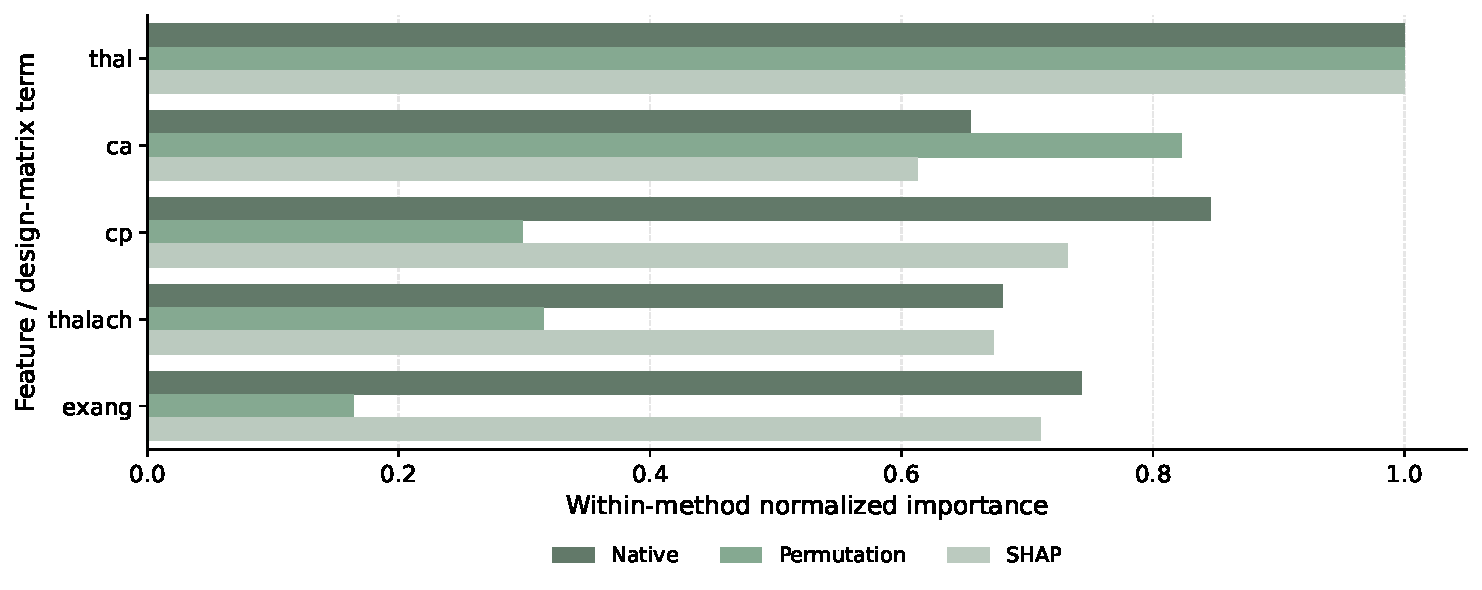
\includegraphics[width=\textwidth]{images/results/heart_global_importance.pdf}
    \caption{Normalised global feature importance for Heart under native importance, permutation importance, and \gls{shap}. Values are normalised independently using the maximum from each method. The five displayed features are selected by mean normalised importance across methods. Bars represent within-method relative importance and not directly comparable raw effects.}
    \label{fig:global_heart}
\end{figure}

\Needspace{10\baselineskip}
\subsection{Stroke}

Age was the leading feature under all three methods and was clearly separated from the remaining variables in the permutation and \gls{shap} results. Average glucose level, the \gls{bmi}-missingness indicator, and heart disease also appeared in the top five under all three methods. Hypertension ranked prominently under native importance and \gls{shap}, while permutation importance instead included the encoded \texttt{ever\_married\_No} term among its five highest-ranked features.

As shown in Figure~\ref{fig:global_stroke}, the strong prominence of age represents model reliance within this dataset and preprocessing configuration. It does not establish a causal effect or remove the influence of the class-weighted modelling procedure described in Chapter~\ref{chap:validation_results} \citep{vilone_classification_2021}.

\begin{figure}[H]
    \centering
    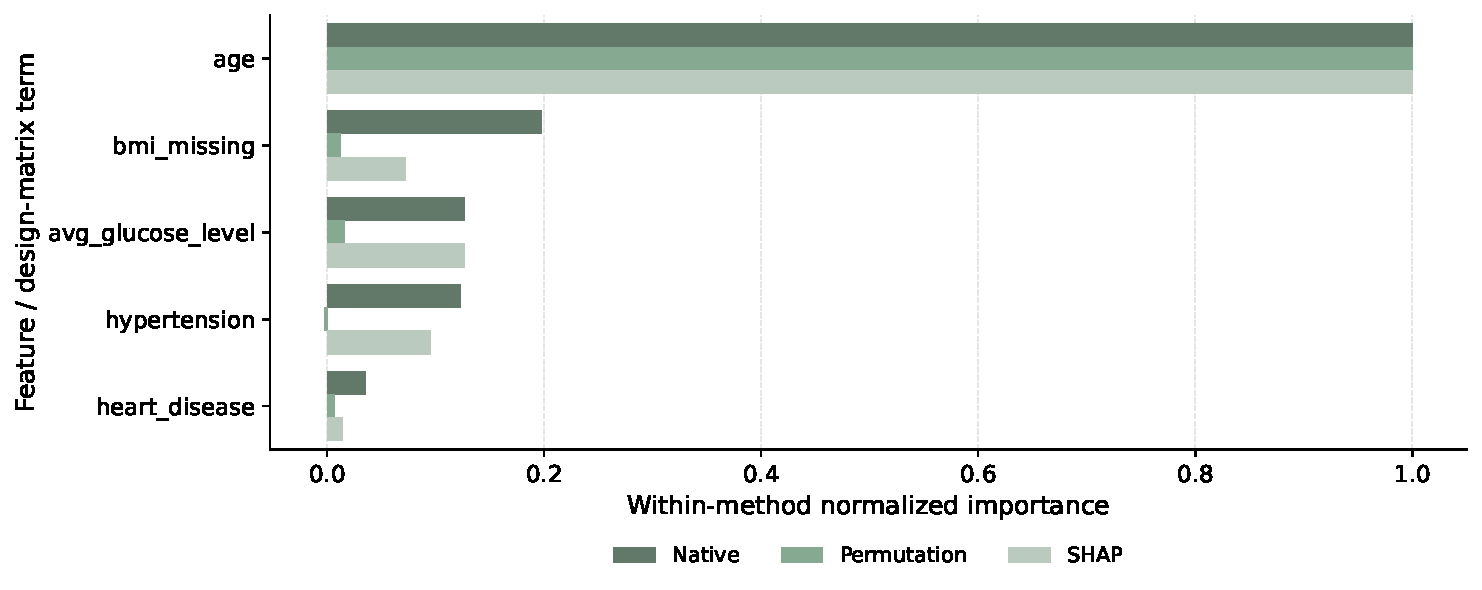
\includegraphics[width=\textwidth]{images/results/stroke_global_importance.pdf}
    \caption{Normalised global feature importance for Stroke under native importance, permutation importance, and \gls{shap}. Values are normalised independently using the maximum from each method. The five displayed features are selected by mean normalised importance across methods. Bars represent within-method relative importance and not directly comparable raw effects.}
    \label{fig:global_stroke}
\end{figure}

\subsection{Diabetes}

The five-feature diabetes \gls{rf} produced the same complete ordering under native importance, permutation importance, and \gls{shap}. Glucose ranked first, followed by \gls{bmi}, age, insulin, and skin thickness.

Figure~\ref{fig:global_diabetes} shows this identical ordering. Because the model contains exactly five predictors, a top-five set overlap of 1.0 is guaranteed when all methods provide importance values for every predictor. The informative finding is therefore the identical ordering rather than complete top-five membership alone. This distinction prevents the overlap statistic from overstating agreement in a model containing only five features.

\begin{figure}[H]
    \centering
    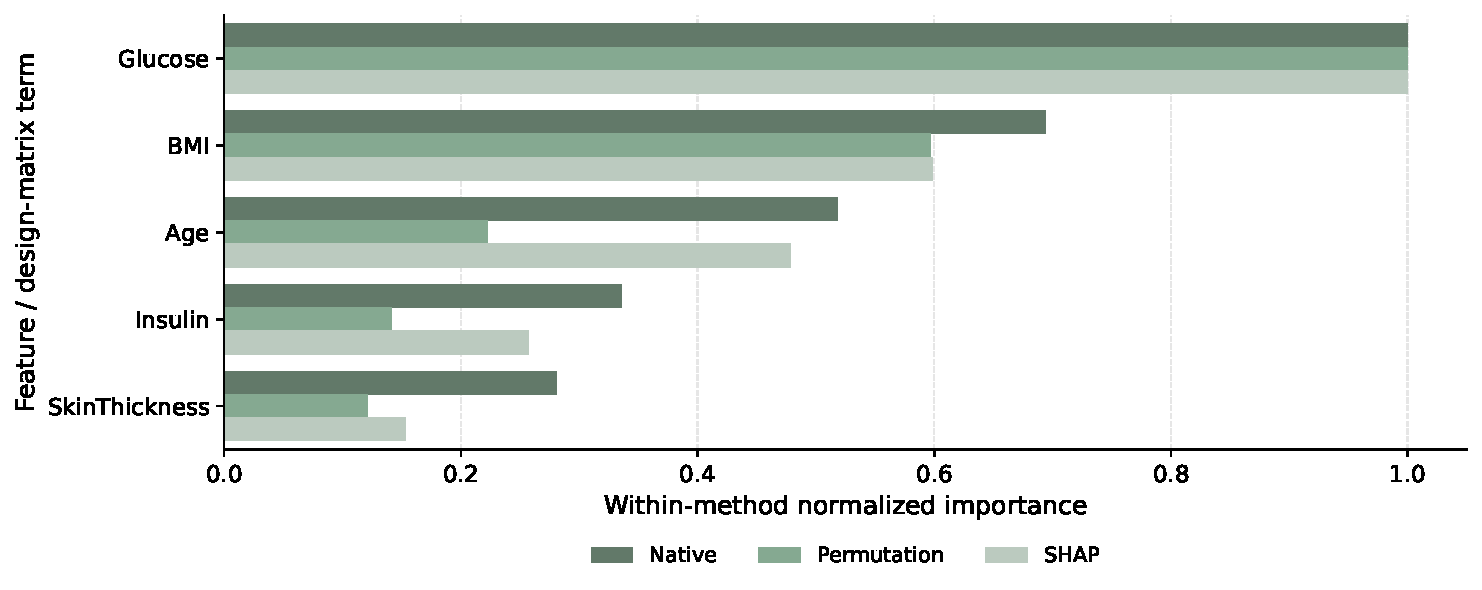
\includegraphics[width=\textwidth]{images/results/diabetes_global_importance.pdf}
    \caption{Normalised global feature importance for Diabetes under native importance, permutation importance, and \gls{shap}. Values are normalised independently using the maximum from each method. The five displayed features are selected by mean normalised importance across methods. Bars represent within-method relative importance and not directly comparable raw effects.}
    \label{fig:global_diabetes}
\end{figure}

\subsection{Chronic Kidney Disease}

Serum creatinine (\emph{sc}), specific gravity (\emph{sg}), haemoglobin (\emph{hemo}), packed cell volume (\emph{pcv}), and albumin (\emph{al}) dominated the native and \gls{shap} results. Native importance ranked serum creatinine first, while permutation importance and \gls{shap} ranked specific gravity first. Specific gravity, serum creatinine, packed cell volume, and albumin appeared in the top five under all three methods.

Figure~\ref{fig:global_ckd} also shows that permutation importance was concentrated on specific gravity, followed by serum creatinine and packed cell volume. Haemoglobin remained prominent under native importance and \gls{shap} but had near-zero permutation importance under the common \gls{rocauc} scorer. The model could therefore assign haemoglobin substantial structural and attribution importance without its isolated permutation materially reducing held-out discrimination. Several lower-ranked variables also remained close to zero, so their relative ordering should not be overinterpreted \citep{fisher_models_2019}.

\begin{figure}[htbp]
    \centering
    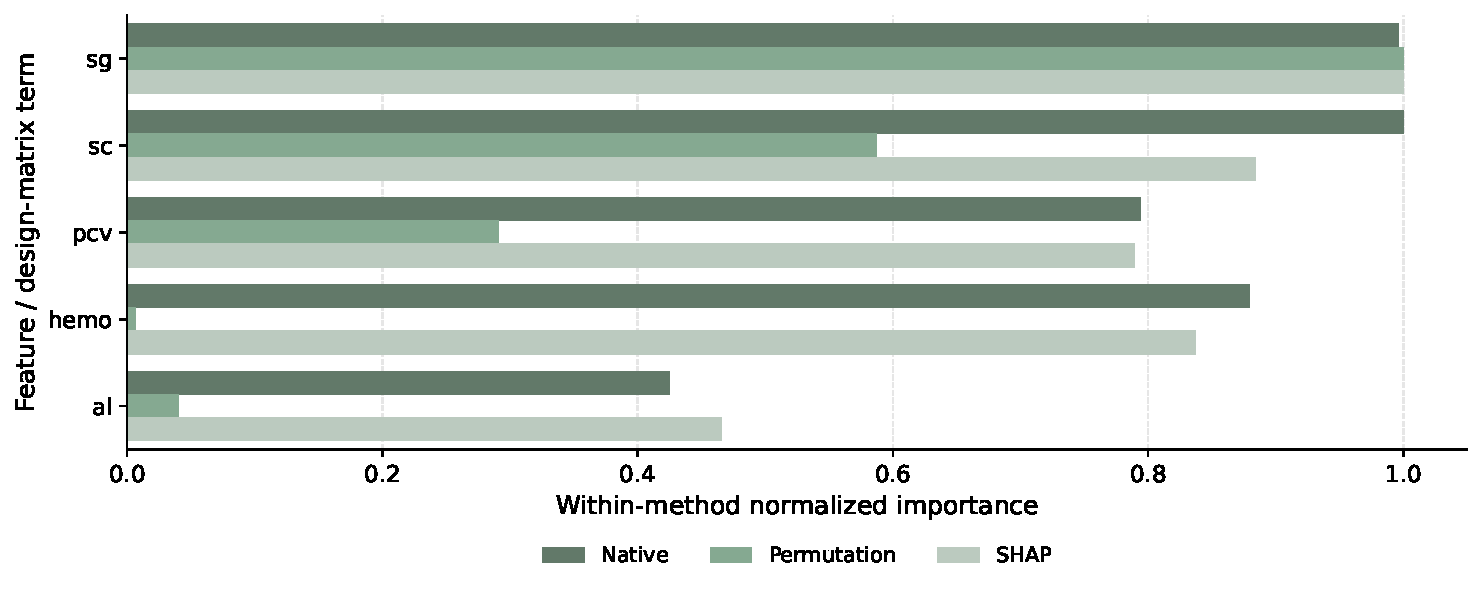
\includegraphics[width=\textwidth]{images/results/ckd_global_importance.pdf}
    \caption{Normalised global feature importance for \gls{ckd} under native importance, permutation importance, and \gls{shap}. Values are normalised independently using the maximum from each method. The five displayed features are selected by mean normalised importance across methods. Bars represent within-method relative importance and not directly comparable raw effects.}
    \label{fig:global_ckd}
\end{figure}
\FloatBarrier

\subsection{\gls{hbaone} and Hospital Readmission}

The \gls{hbaone} model exhibited the clearest separation between estimator-specific coefficients and model-agnostic importance. Native coefficient magnitude was dominated by interactions between medical specialty and the youngest age group. The largest absolute coefficient corresponded to the interaction between surgery specialty and age 30 years or younger. In contrast, permutation importance and \gls{shap} both ranked time in hospital first, followed by missing or unknown specialty and the non-home-discharge indicator.

Figure~\ref{fig:global_hba1c} uses mean normalised importance across all three methods to select the five displayed terms. This rule was used to provide a balanced cross-method summary rather than reproduce the top-five set from one method. Consequently, the non-home-discharge term was not displayed even though it ranked highly under permutation importance and \gls{shap}. Its lower native ranking reduced its mean normalised importance across the three methods.

Permutation importance and \gls{shap} shared four of their five highest-ranked terms. Native importance shared none of its top five with either model-agnostic set. This divergence is consistent with the different quantities measured by the methods. Native ranking uses absolute coefficient magnitude, which is sensitive to feature scale, categorical coding, and the frequency of encoded terms. Permutation importance measures the reduction in \gls{rocauc} after a design column is disrupted, while aggregated \gls{shap} measures average attribution magnitude across observations \citep{fisher_models_2019, NIPS2017_8a20a862}. A large coefficient associated with a rare design term can therefore have limited average permutation or \gls{shap} importance.

\begin{figure}[H]
    \centering
    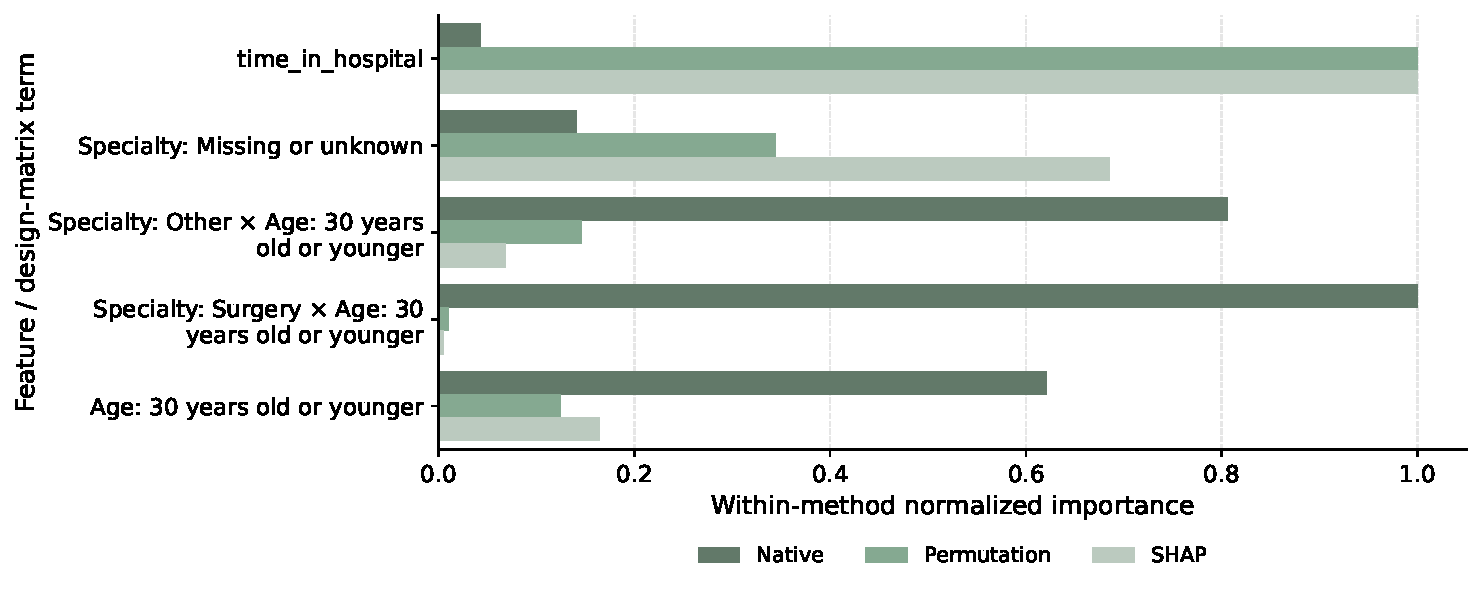
\includegraphics[width=\textwidth]{images/results/hba1c_global_importance.pdf}
    \caption{Normalised global feature importance for \gls{hbaone} under native importance, permutation importance, and \gls{shap}. Values are normalised independently using the maximum from each method. The five displayed terms are selected by mean normalised importance across methods. Bars represent within-method relative importance and not directly comparable raw effects.}
    \label{fig:global_hba1c}
\end{figure}

\subsection{Top-Five Synthesis}

Table~\ref{tab:global_top5_overlap} compares pairwise overlap among the top-five feature sets. N--S denotes native importance compared with \gls{shap}, N--P denotes native importance compared with permutation importance, and S--P denotes \gls{shap} compared with permutation importance. The Common column reports the number of features appearing in the top five under all three methods.

\begin{table}[H]
    \centering
    \small
    \caption{Pairwise overlap among the five highest-ranked features produced by the global \gls{xai} methods. N-S denotes native importance versus \gls{shap}, N-P denotes native importance versus permutation importance, and S-P denotes \gls{shap} versus permutation importance.}
    \label{tab:global_top5_overlap}
    \begin{tabular}{@{}lrrrrl@{}}
        \toprule
        \textbf{Dataset} & \textbf{N--S} & \textbf{N--P} & \textbf{S--P} & \textbf{Common} & \textbf{Features common to all} \\
        \midrule
        Heart & 0.80 & 0.80 & 0.60 & 3 & thal, cp, thalach \\
        Stroke & 1.00 & 0.80 & 0.80 & 4 & age, glucose, \gls{bmi} missing, heart disease \\
        Diabetes & 1.00 & 1.00 & 1.00 & 5 & all five model predictors \\
        \gls{ckd} & 1.00 & 0.80 & 0.80 & 4 & al, pcv, sc, sg \\
        \gls{hbaone} & 0.00 & 0.00 & 0.80 & 0 & none \\
        \bottomrule
    \end{tabular}
\end{table}

Top-feature agreement varied across datasets. Complete set-level agreement occurred only for the five-feature diabetes model, where inclusion of all predictors was unavoidable. Heart, Stroke, and \gls{ckd} retained shared feature cores while differing in the remaining top-ranked features. \gls{hbaone} showed strong top-five overlap between \gls{shap} and permutation importance but no top-five overlap between native importance and either model-agnostic method.

\section{Agreement Between Global \gls{xai} Methods}

Spearman rank correlation was calculated after aligning features by name and assigning average ranks to tied importance values \citep{spearman_proof_1904}. Table~\ref{tab:rank_agreement} provides the numerical correlations, while Figure~\ref{fig:method_agreement} displays the same results across datasets and method pairs.

\begin{table}[htbp]
    \centering
    \small
    \caption{Spearman rank agreement among native importance, permutation importance, and \gls{shap} across all aligned features in each analytical configuration. Values closer to one indicate greater similarity between the corresponding feature rankings.}
    \label{tab:rank_agreement}
    \begin{tabular}{@{}lrrrr@{}}
        \toprule
        \textbf{Dataset} & \textbf{Features} & \textbf{Native-\gls{shap}} & \textbf{Native-Permutation} & \textbf{\gls{shap}-Permutation} \\
        \midrule
        Heart & 13 & 0.978 & 0.621 & 0.615 \\
        Stroke & 7 & 0.893 & 0.739 & 0.631 \\
        Diabetes & 5 & 1.000 & 1.000 & 1.000 \\
        \gls{ckd} & 24 & 0.981 & 0.728 & 0.741 \\
        \gls{hbaone} & 90 & 0.047 & 0.409 & 0.883 \\
        \bottomrule
    \end{tabular}
\end{table}

Heart and \gls{ckd} showed near-perfect agreement between native and \gls{shap} rankings. Agreement involving permutation importance was moderate for Heart and moderately high for \gls{ckd}. Stroke followed the same general pattern, although its native--\gls{shap} correlation was lower. Diabetes produced identical ranks across all methods. \gls{hbaone} showed the reverse pattern. \gls{shap} and permutation importance were strongly correlated at $\rho=0.883$, while native importance and \gls{shap} were almost uncorrelated at $\rho=0.047$. These values are visualised in Figure~\ref{fig:method_agreement}.

\begin{figure}[htbp]
    \centering
    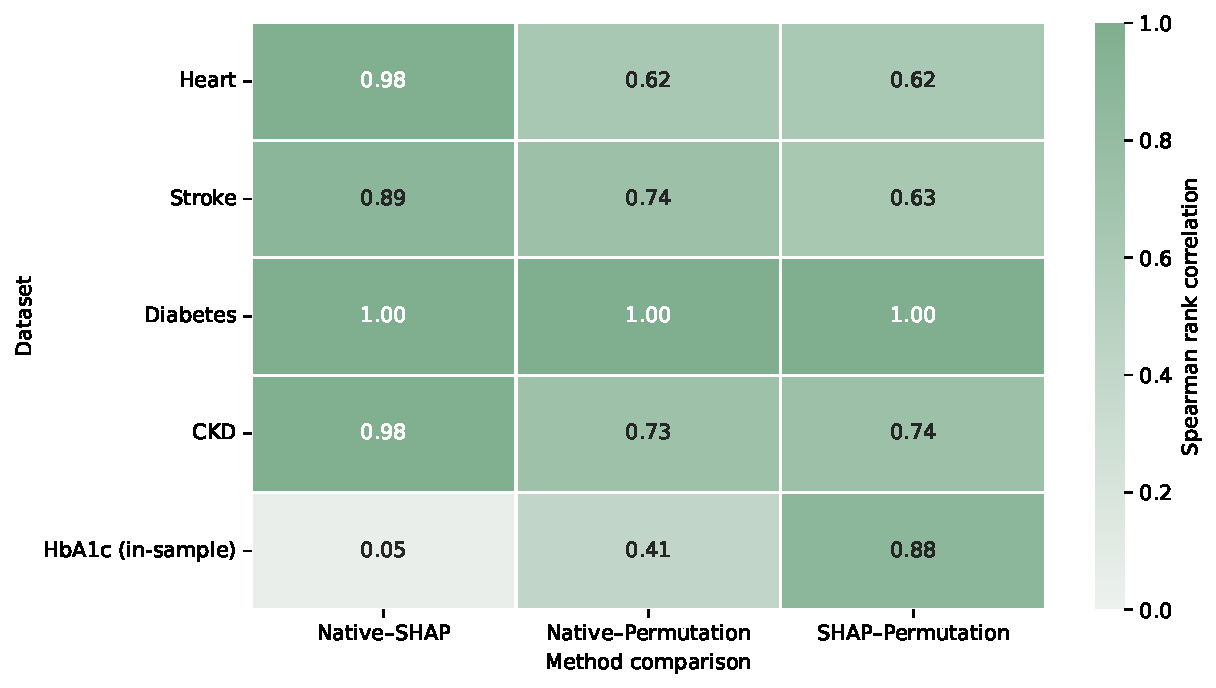
\includegraphics[width=\textwidth]{images/results/rank_agreement_heatmap.pdf}
    \caption{Spearman rank agreement among native importance, permutation importance, and \gls{shap} across all aligned features in each dataset. Cell values and colour intensity represent the correlation between each pair of feature rankings, with higher values indicating greater agreement.}
    \label{fig:method_agreement}
\end{figure}

For \gls{hbaone}, absolute logistic-regression coefficients depend on the scale, coding, and prevalence of the corresponding design terms. Sparse categorical levels and interactions can receive large coefficients without making large average contributions across the cohort \citep{linardatos_explainable_2020, vilone_classification_2021}. The weak native-\gls{shap} correlation therefore does not by itself indicate an implementation inconsistency. Similarly, permutation of an individual expanded design column measures reliance on that encoded term within the fitted model. It should not be interpreted as a clinical intervention \citep{fisher_models_2019}.

These findings answer RQ2 by showing that agreement depends on the dataset, model representation, and quantity measured by each explanation method. Native importance and \gls{shap} were closely aligned for the linear and tree-based predictive configurations, while permutation rankings diverged more frequently. In the interaction-rich \gls{hbaone} model, the two aggregated model-agnostic methods agreed strongly with each other but not with absolute coefficient magnitude. Agreement between explanation methods must therefore be interpreted in relation to model structure and method-specific definitions \citep{vilone_classification_2021, lofstrom_meta_2022}.

\section{Stability of Global Explanations}

Bootstrap-refit stability was evaluated for Heart, Stroke, Diabetes, and \gls{ckd} using 100 stratified bootstrap samples of each final training matrix. A new model was fitted to each bootstrap sample, while permutation importance was evaluated on the fixed held-out test set using negative log loss. This produced 4,950 pairwise ranking comparisons per dataset. Table~\ref{tab:stability_results} reports the mean Spearman correlation, mean overlap among the three highest-ranked features, and the features that appeared most frequently in the top three. Figure~\ref{fig:stability_ranks} presents the two stability measures together.

\begin{table}[htbp]
    \centering
    \small
    \caption{Bootstrap-refit stability of global permutation-importance rankings in the principal analysis. Mean values were calculated across all 4,950 pairs of rankings obtained from 100 successful bootstrap refits.}
    \label{tab:stability_results}
    \begin{tabular}{@{}lrrrl@{}}
        \toprule
        \textbf{Dataset} & \textbf{Mean $\rho$} & \textbf{Mean top-3 overlap} & \textbf{Comparisons} & \textbf{Most persistent features} \\
        \midrule
        Heart & 0.700 & 0.645 & 4,950 & ca, thal \\
        Stroke & 0.812 & 0.741 & 4,950 & age, marital status \\
        Diabetes & 0.849 & 0.890 & 4,950 & glucose, \gls{bmi} \\
        \gls{ckd} & 0.949 & 0.759 & 4,950 & specific gravity, packed cell volume \\
        \gls{hbaone} & -- & -- & 0 & not included \\
        \bottomrule
    \end{tabular}
\end{table}

\begin{figure}[H]
    \centering
    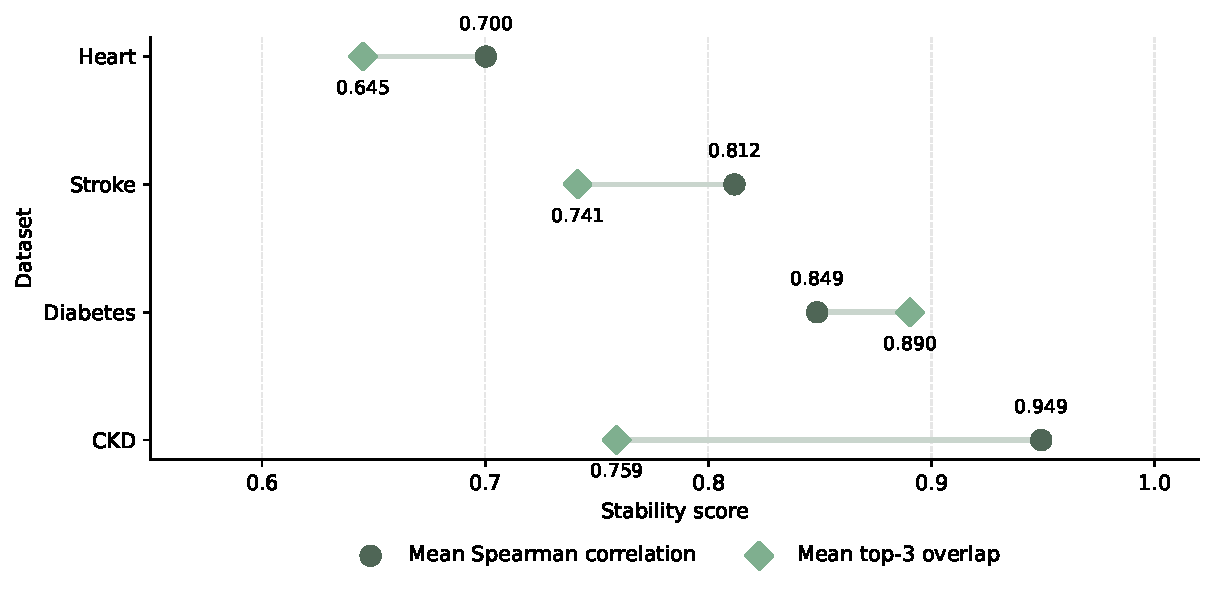
\includegraphics[width=\textwidth]{images/results/stability_combined.pdf}
    \caption{Bootstrap-refit stability of permutation-importance rankings in the principal analysis. Circles show the mean pairwise Spearman correlation and diamonds show the mean top-three overlap across the 4,950 pairs of rankings obtained from 100 bootstrap refits. Permutation importance was evaluated on the fixed held-out test set using negative log loss. \gls{hbaone} was excluded because only 58 of 100 refits converged in its exploratory grouped-permutation sensitivity experiment.}
    \label{fig:stability_ranks}
\end{figure}

Heart had the lowest complete-ranking stability of the four evaluated datasets, with a mean Spearman correlation of 0.700 and mean top-three overlap of 0.645. The most persistent Heart features were \emph{ca} and \emph{thal}, which appeared among the three highest-ranked features in 91\% and 77\% of bootstrap refits, respectively. Stroke showed stronger persistence, with a mean correlation of 0.812 and top-three overlap of 0.741. Age appeared in the top three in every Stroke refit, while the two encoded marital-status columns also appeared frequently.

Diabetes produced a mean rank correlation of 0.849 and the highest top-three overlap, 0.890. Glucose appeared in the top three in every refit and \gls{bmi} did so in 91\% of refits. \gls{ckd} produced the highest complete-ranking stability, with a mean correlation of 0.949, while its mean top-three overlap was 0.759. Specific gravity appeared in the top three in every \gls{ckd} refit and packed cell volume did so in 82\% of refits. The revised probability-based analysis therefore did not reproduce the low \gls{ckd} stability observed under accuracy scoring, where the small test set produced coarse score changes and many tied importances.

No \gls{hbaone} estimate was included in the principal stability comparison because its canonical analytical bundle did not contain a validated retraining callback capable of producing equivalent refits. Substituting a different model or preprocessing procedure would have evaluated another analytical workflow.

An exploratory grouped-permutation bootstrap analysis was subsequently attempted using a reconstructed Statsmodels retraining procedure. Computational runtime was feasible, but only 58 of 100 bootstrap refits converged. The resulting stability estimate was not incorporated into the principal analysis because excluding the 42 failed refits could introduce selection bias. The exploratory output was retained as sensitivity evidence, while \gls{hbaone} stability remains a limitation of the study.

RQ4 is answered for the four retrainable predictive configurations. Bootstrap-refit rankings showed moderate-to-strong persistence, but the ordering differed by dataset and by whether stability was assessed over the complete ranking or only the three leading features. These findings apply specifically to changes in the composition of the final training matrix under a fixed test set and fixed permutation procedure \citep{lofstrom_meta_2022, canha_functionally-grounded_2025}.

\section{Local Explanations and Representative Cases}

\subsection{Case Availability}

Representative cases were selected to examine local model behaviour across different prediction outcomes. The procedure considered \glspl{tp}, \glspl{tn}, \glspl{fp}, \glspl{fn}, and observations closest to the classification threshold that had not already been selected under another case type. Up to ten observations were retained per available category. This outcome-based selection provides multiple examples of successful, unsuccessful, and boundary predictions, but it does not produce a random or population-representative sample \citep{ribeiro_why_2016, vilone_classification_2021}.

Table~\ref{tab:local_case_availability} shows which case types were available for each analytical configuration.

\begin{table}[htbp]
    \centering
    \small
    \renewcommand{\arraystretch}{1.15}
    \caption{Numbers of observations included in the repeated \gls{lime} analysis at the classification threshold of 0.5. A dash indicates that the corresponding prediction outcome was unavailable.}
    \label{tab:local_case_availability}
    \begin{tabular}{@{}lccccc@{}}
        \toprule
        \textbf{Dataset} & \textbf{\gls{tp}} & \textbf{\gls{tn}} & \textbf{\gls{fp}} & \textbf{\gls{fn}} & \textbf{Borderline} \\
        \midrule
        Heart & 10 & 10 & 10 & 10 & 10 \\
        Stroke & 10 & 10 & 10 & 10 & 10 \\
        Diabetes & 10 & 10 & 10 & 10 & 10 \\
        \gls{ckd} & 10 & 10 & 1 & 1 & 10 \\
        \gls{hbaone} & -- & 10 & -- & 10 & 10 \\
        \bottomrule
    \end{tabular}
\end{table}





Heart, Stroke, and Diabetes contributed ten observations to each category. \gls{ckd} contributed ten true positives, ten true negatives, and ten borderline observations, but its held-out predictions contained only one false positive and one false negative; both errors were retained. The resulting comparison therefore remains descriptive and is unbalanced for the \gls{ckd} error categories.

The \gls{hbaone} model produced no positive classifications at the threshold of 0.5. Consequently, no \gls{tp} or \gls{fp} case was available. Its closest observation to the threshold had a predicted probability of 0.353. It is retained as the operational borderline case because it was the closest available observation, although it was not close to 0.5 in absolute terms. This outcome is consistent with the in-sample inferential role of the \gls{hbaone} configuration and should not be interpreted as evidence of a clinically validated decision threshold.

\subsection{Illustrative \gls{lime} Results}

\gls{lime} explanations describe the behaviour of a fitted local surrogate around an individual observation. Each selected observation was explained using 20 perturbation seeds. Case-level rule weights were averaged over those seeds, while seed-to-seed rank agreement, top-three overlap, weight dispersion, and sign consistency were retained as sensitivity measures. Their rules and weights should still be interpreted as case-specific approximations rather than as population-level effects or causal relationships \citep{ribeiro_why_2016, vilone_classification_2021}.

Table~\ref{tab:lime_seed_stability} summarises sensitivity to the perturbation seed across all selected observations. Mean pairwise rank correlations ranged from 0.898 for \gls{ckd} to 0.969 for Stroke, and mean top-three overlap ranged from 0.892 for \gls{hbaone} to 0.998 for Stroke. The leading local rules were therefore generally persistent across seeds. Mean sign consistency was lower for Stroke and \gls{hbaone} because small or intermittently selected rules could change direction even when the leading-rule ordering remained similar. Weight standard deviations are reported for completeness but should be compared only within a dataset because raw \gls{lime} scales depend on the fitted model and representation.

\begin{table}[htbp]
    \centering
    \small
    \caption{Stability of repeated \gls{lime} explanations across 20 perturbation seeds. Values are means across the selected observations in each dataset. Rank correlation is the mean pairwise Spearman correlation between seed-specific rule rankings; top-three overlap is the mean proportion of shared rules among the three largest absolute weights.}
    \label{tab:lime_seed_stability}
    \begin{tabular}{@{}lrrrrr@{}}
        \toprule
        \textbf{Dataset} & \textbf{Cases} & \textbf{Rank $\rho$} & \textbf{Top-3 overlap} & \textbf{Weight SD} & \textbf{Sign consistency} \\
        \midrule
        Heart & 50 & 0.963 & 0.954 & 0.003 & 0.900 \\
        Stroke & 50 & 0.969 & 0.998 & 0.009 & 0.815 \\
        Diabetes & 50 & 0.956 & 0.926 & 0.007 & 1.000 \\
        \gls{ckd} & 32 & 0.898 & 0.919 & 0.007 & 0.871 \\
        \gls{hbaone} & 30 & 0.944 & 0.892 & 0.027 & 0.799 \\
        \bottomrule
    \end{tabular}
\end{table}

For Heart, chest-pain type was the strongest \gls{lime} rule in all five representative cases. Its contribution changed direction according to the discretised interval. Lower chest-pain coding supported the negative class, while an intermediate interval supported the positive class. The rule appeared in correct predictions and errors. Its presence alone therefore did not distinguish successful from unsuccessful predictions. Because \texttt{cp} was retained as a source-coded nominal variable, these numerical intervals describe regions of the reproduced model input and must not be interpreted as ordered clinical categories or meaningful clinical cut-offs.

For Stroke, age dominated the \gls{tp}, \gls{tn}, \gls{fp}, and \gls{fn} explanations. Older age strongly supported the positive class for both the \gls{tp} and the high-confidence \gls{fp}. Younger age strongly supported the negative class for both the \gls{tn} and \gls{fn}. The borderline explanation was instead led by the \gls{bmi}-missingness indicator. The \gls{fp} had a predicted probability of 0.986, while the \gls{fn} had a predicted probability of 0.024. These cases demonstrate that prediction errors were not restricted to observations near the decision threshold.

Figure~\ref{fig:representative_lime_stroke} compares the five representative Stroke explanations. Age made the strongest positive contribution in both the \gls{tp} and \gls{fp} cases. Younger age and a lower value of the \gls{bmi}-missingness indicator contributed towards the negative class in the \gls{tn} and \gls{fn} cases. These explanations illustrate local decision behaviour and do not represent population-level feature effects.

\begin{sidewaysfigure}[p]
    \centering
    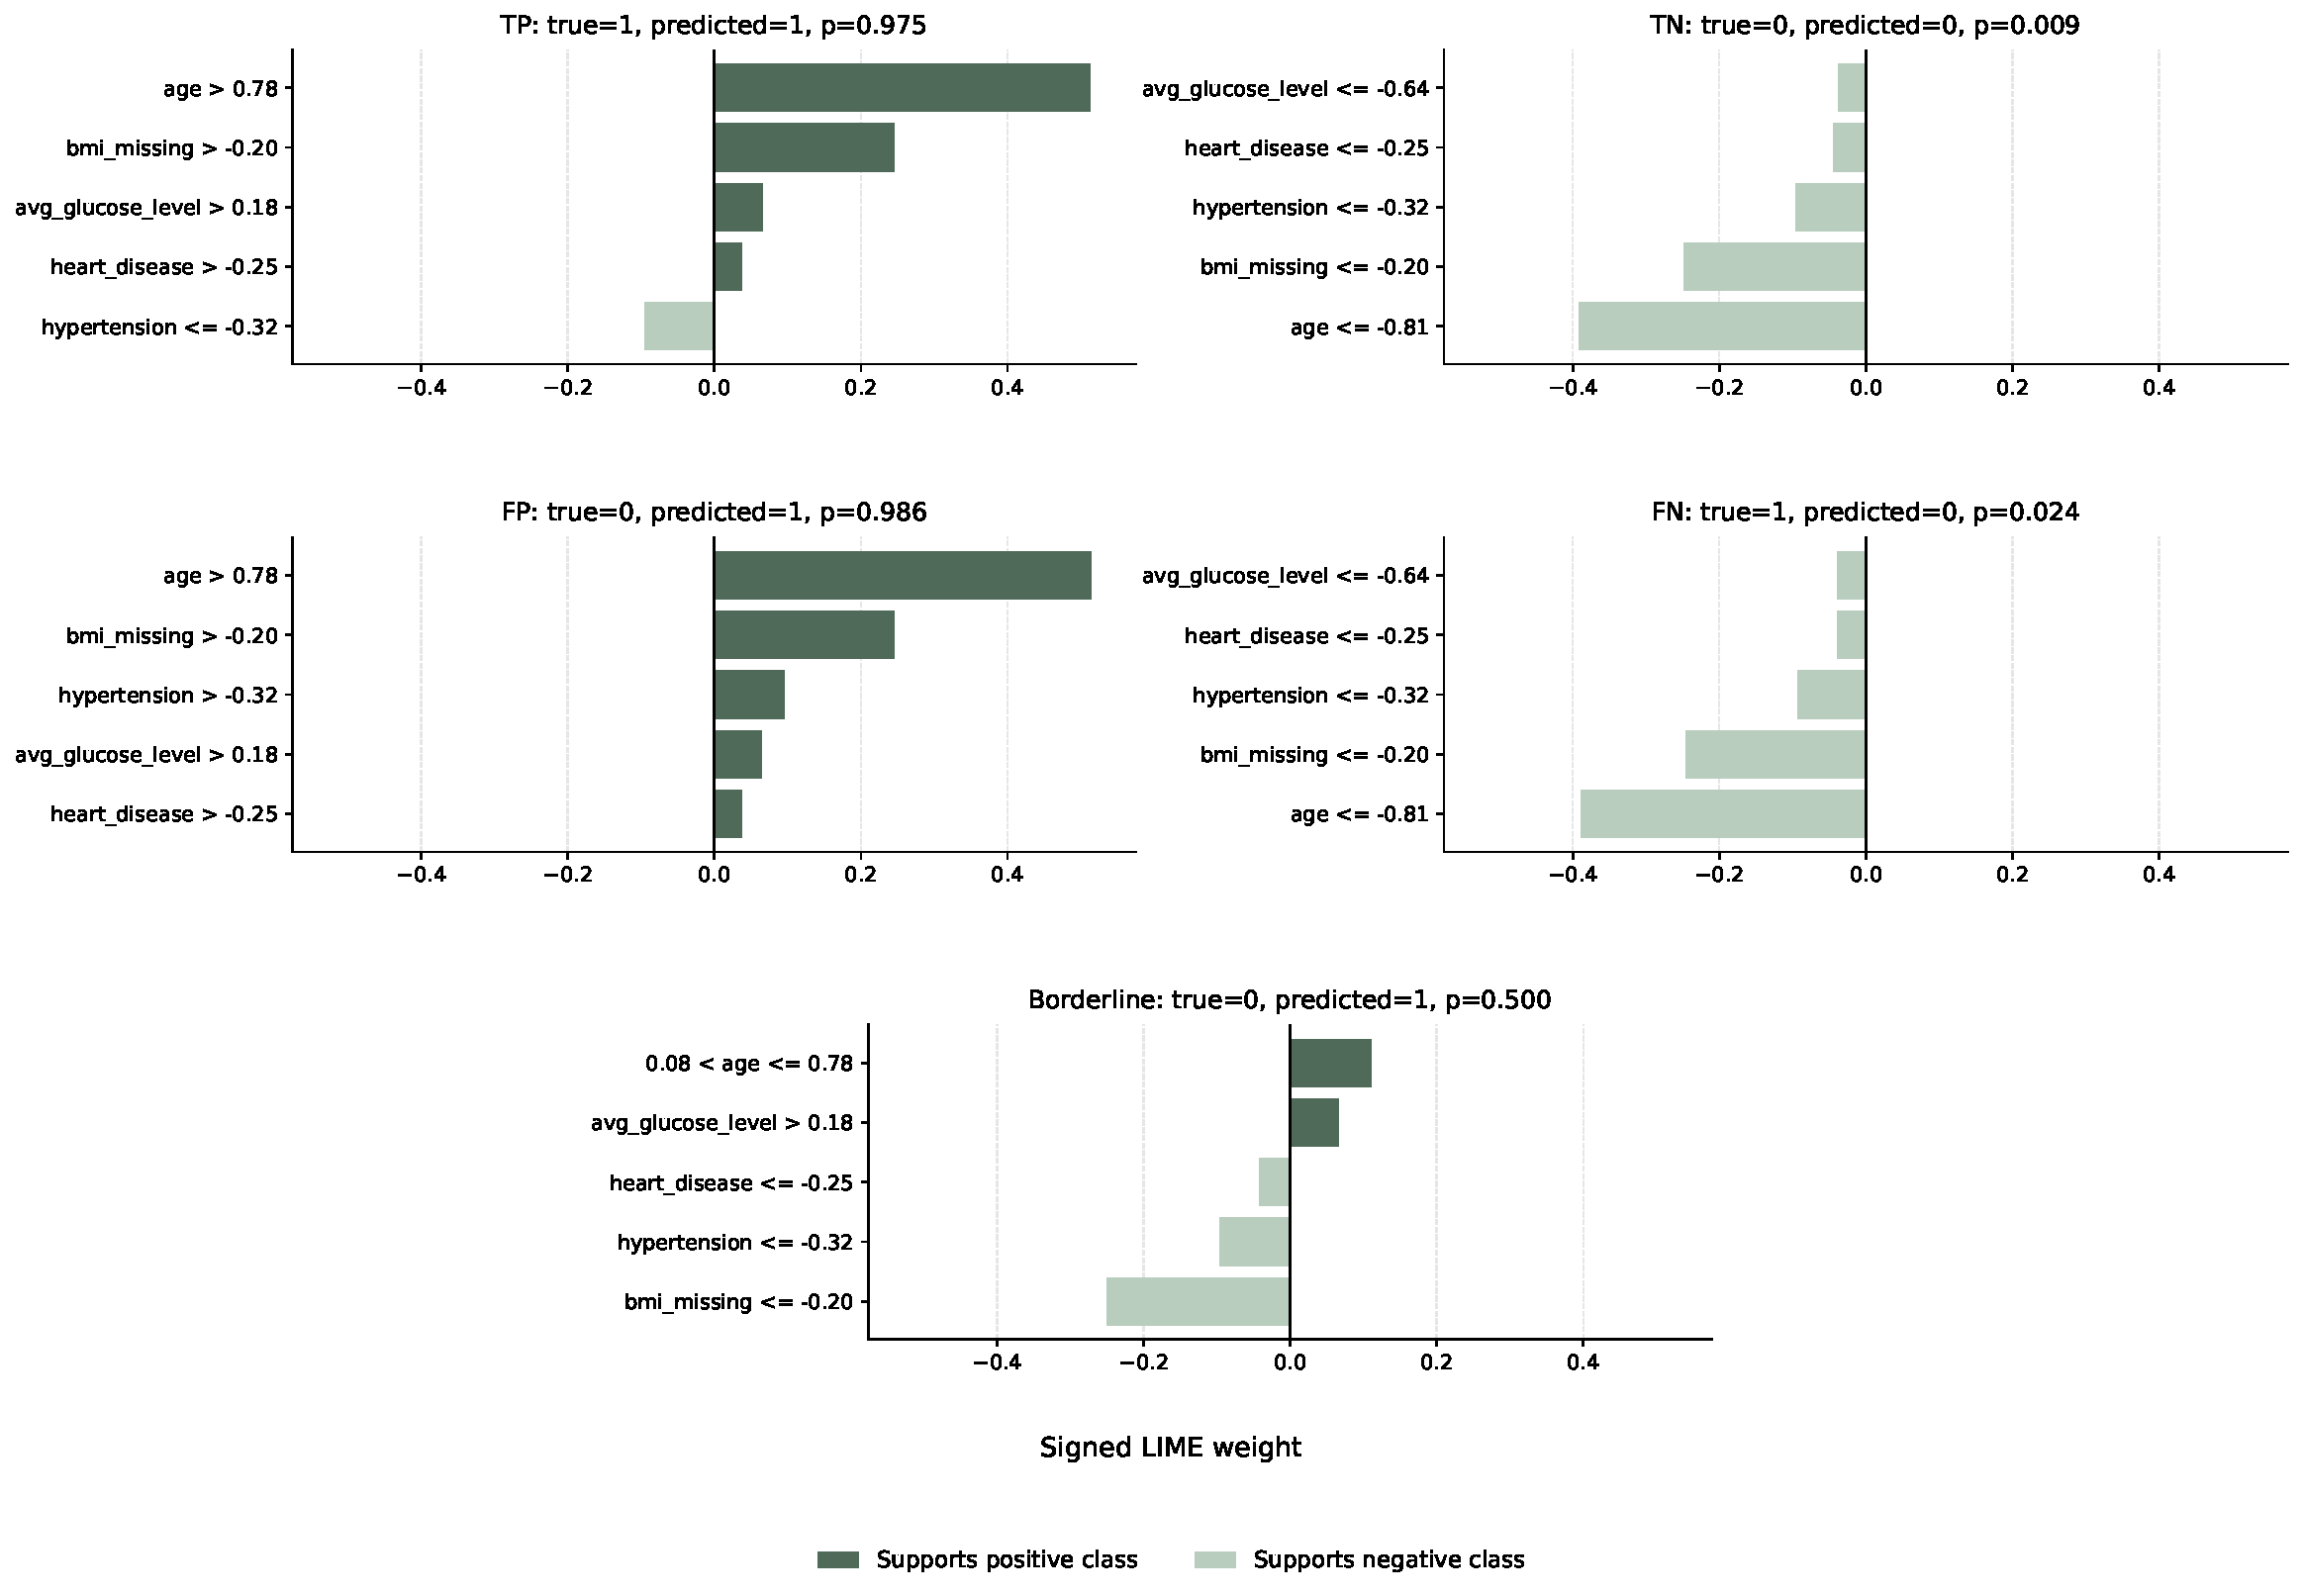
\includegraphics[
        width=0.92\textheight
    ]{images/results/stroke_representative_lime.pdf}
    \caption{Illustrative local \gls{lime} explanations for the highest-ranked Stroke observation in each case category. Bars show signed weights averaged across 20 perturbation seeds. Dark bars support the positive class, while light bars support the negative class. \gls{lime} weights describe fitted local surrogates and are not calibrated clinical effect sizes.}
    \label{fig:representative_lime_stroke}
\end{sidewaysfigure}

The corresponding Heart explanations are presented in Figure~\ref{fig:representative_lime_heart} in Appendix~\ref{app:local_explanations}. The Diabetes, \gls{ckd}, and \gls{hbaone} explanations are presented in Figures~\ref{fig:representative_lime_diabetes}, \ref{fig:representative_lime_ckd}, and \ref{fig:representative_lime_hba1c}, respectively.

In Diabetes, high glucose was the strongest positive rule for both the \gls{tp} and \gls{fp}, while low glucose supported the \gls{tn}. The \gls{fn} was led by a low-\gls{bmi} rule, and the borderline prediction was led by high \gls{bmi}. Figure~\ref{fig:representative_lime_diabetes} shows that glucose and \gls{bmi} contributed to both correct and incorrect predictions under different local conditions.

In \gls{ckd}, serum creatinine led the \gls{tp} and \gls{fp} explanations, while packed cell volume and haemoglobin led the \gls{tn} and \gls{fn} explanations, respectively. As shown in Figure~\ref{fig:representative_lime_ckd}, similar local rules could occur in correct and incorrect predictions.

The three illustrative \gls{hbaone} cases were led by the same absent interaction indicator involving the ``Other'' specialty category and age 30 years or younger. Figure~\ref{fig:representative_lime_hba1c} also shows that the \gls{hbaone} weights were numerically larger than those in the other datasets. This does not indicate stronger or more reliable explanations. \gls{lime} magnitudes depend on the feature representation, perturbation distribution, proximity weighting, and fitted local surrogate \citep{ribeiro_why_2016}. The encoded interaction terms are also less directly interpretable than raw clinical measurements.

\subsection{Local Explanation Magnitude by Case and Outcome}

Figure~\ref{fig:lime_case_type} summarises relative local explanation magnitude by representative case type. Values were normalised independently within each dataset using its largest mean absolute \gls{lime} weight. Missing case types were omitted because no corresponding representative case and explanation existed. Assigning zero would incorrectly represent absence of a case as an observed explanation with zero magnitude.

Raw absolute \gls{lime} weights are interpreted only within each dataset and fitted model. Their magnitudes depend on the local representation, perturbation procedure, proximity weighting, and fitted surrogate \citep{ribeiro_why_2016}. The larger raw \gls{hbaone} weights therefore do not demonstrate greater explanation fidelity or clinical relevance. Normalisation supports comparison of case-type patterns within each dataset, but it does not create a common scale across datasets.

The selected cases are deliberately chosen examples rather than random samples from their outcome groups. The summaries average up to ten selected observations per category after first averaging each observation's rule weights across 20 seeds. This broader design reduces dependence on one observation and one perturbation sequence, but the selected cases still cannot support population-level conclusions about differences between correct and erroneous predictions.


\begin{figure}[H]
    \centering
    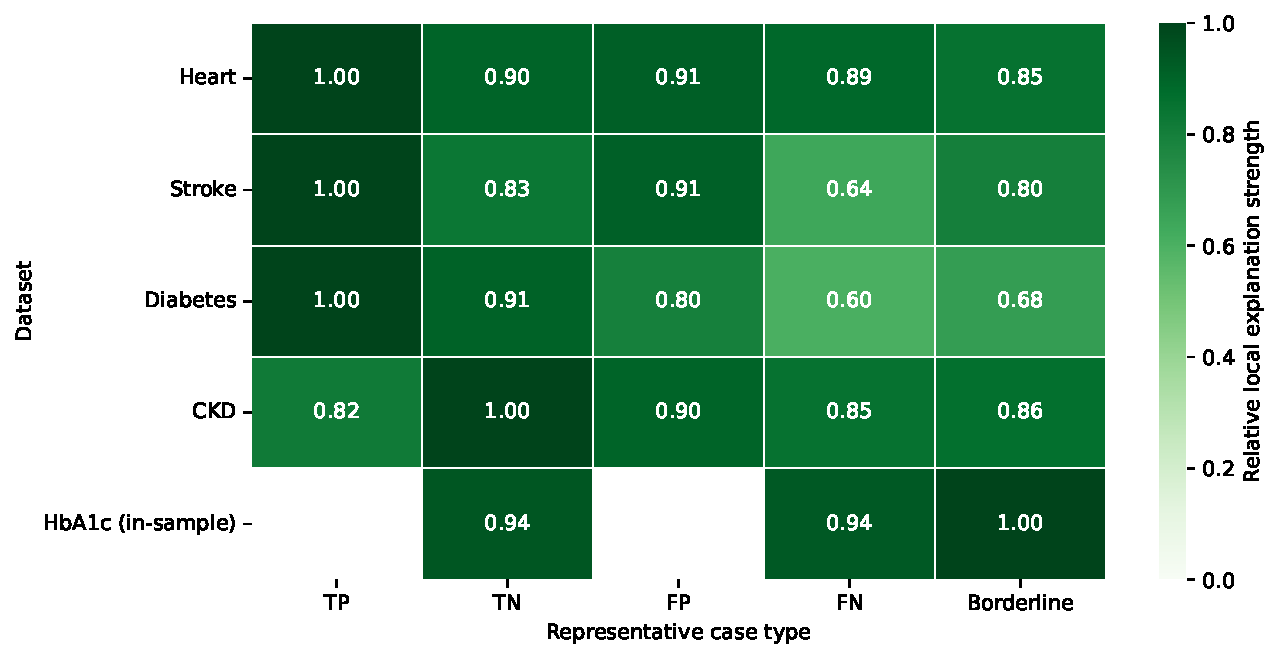
\includegraphics[width=0.90\textwidth]
    {images/results/lime_case_type_normalized_v2.pdf}
    \caption{Relative mean absolute \gls{lime} weight by representative case type. Case-level weights were first averaged across 20 perturbation seeds and then summarised over all available selected observations. Values are normalised independently within each dataset using its largest available value. Empty cells indicate that no case of that type was available and are not zero values.}
    \label{fig:lime_case_type}
\end{figure}

\FloatBarrier

\subsection{Global-Local Feature Presence}

Global-local feature presence was defined as the proportion of the five highest-ranked global \gls{shap} features whose names appeared among the five strongest seed-averaged \gls{lime} rules for a selected observation. The resulting means and observed ranges are presented in Table~\ref{tab:global_local_overlap}. This analysis evaluates lexical feature presence rather than equivalence between \gls{shap} and \gls{lime}, which have different explanation definitions \citep{NIPS2017_8a20a862, ribeiro_why_2016, vilone_classification_2021}.

Stroke and Diabetes showed the highest global-local feature presence. \gls{ckd} and Heart showed lower overlap, while \gls{hbaone} remained markedly lower. The Diabetes value is structurally inflated because all five predictors in the model belong to the global top-five set. \gls{hbaone} overlap varied from 0.20 to 0.40 across its 30 selected observations, reflecting its sparse interaction-rich design terms.

\begin{table}[htbp]
    \centering
    \small
    \caption{Lexical overlap between the five highest-ranked global \gls{shap} features and the \gls{lime} rule strings of the representative cases. The table reports the number of available cases, mean overlap, and observed range for each dataset.}
    \label{tab:global_local_overlap}
    \begin{tabular}{@{}lrrr@{}}
        \toprule
        \textbf{Dataset} & \textbf{Cases} & \textbf{Mean overlap} & \textbf{Range} \\
        \midrule
        Heart & 50 & 0.724 & 0.60--0.80 \\
        Stroke & 50 & 0.996 & 0.80--1.00 \\
        Diabetes & 50 & 1.000 & 1.00--1.00 \\
        \gls{ckd} & 32 & 0.763 & 0.60--0.80 \\
        \gls{hbaone} & 30 & 0.373 & 0.20--0.40 \\
        \bottomrule
    \end{tabular}
\end{table}

The reported overlap is lexical and is not a formal agreement coefficient between \gls{shap} and \gls{lime}. It does not compare attribution signs, magnitudes, \gls{lime} rule intervals, or the fidelity of the local surrogate.

The findings provide a descriptive answer to RQ3 based on 212 selected observations and 20 perturbation seeds per observation. Local explanations reflected case-specific feature values and could assign different directions to the same feature under different local conditions. Correct and erroneous predictions frequently shared their strongest rules. Prediction confidence was also not consistently associated with correctness, as demonstrated by the confident Stroke \gls{fp} and \gls{fn} cases. Global-local feature presence should therefore be interpreted as evidence that the same feature names occur in both explanation levels, not as evidence that the methods agree about their effects or that a prediction is correct.

Mean absolute \gls{lime} weights were slightly higher for correct cases than for erroneous cases in each dataset where both groups were available. The difference was small, the observations were deliberately selected, and \gls{ckd} contained only two error cases. Raw weights are also not comparable across datasets. These descriptive differences do not support inferential or population-level conclusions.

\section{Cross-Dataset and Model-Family Comparison}

The dataset-level findings differed across global agreement, bootstrap-refit stability, and representative local behaviour. Table~\ref{tab:xai_synthesis} brings these dimensions together so that strong performance in one dimension is not interpreted as evidence of strength in another.

\begin{table}[!t]
    \centering
    \small
    \caption{Synthesis of the key global-agreement, bootstrap-refit stability, and representative local-explanation findings across the five analytical configurations.}
    \label{tab:xai_synthesis}
    \begin{tabularx}{\textwidth}{
        @{}l
        >{\RaggedRight\arraybackslash}X
        >{\RaggedRight\arraybackslash}X
        >{\RaggedRight\arraybackslash}X@{}
    }
        \toprule
        \textbf{Dataset}
        & \textbf{Global agreement}
        & \textbf{Stability}
        & \textbf{Local finding} \\
        \midrule

        Heart
        & Native and \gls{shap} were closely aligned; agreement with
        permutation was moderate.
        & Mean $\rho=0.700$ and top-three overlap $=0.645$; \emph{ca}
        and \emph{thal} were most persistent.
        & Chest-pain rules appeared in correct and incorrect cases;
        mean \gls{lime} seed-rank $\rho=0.963$. \\

        Stroke
        & Native and \gls{shap} showed strong agreement; permutation
        differed more.
        & Mean $\rho=0.812$ and top-three overlap $=0.741$; age and
        marital status were most persistent.
        & Age dominated correct and confident incorrect predictions;
        mean \gls{lime} seed-rank $\rho=0.969$. \\

        Diabetes
        & All three methods produced the same complete ordering.
        & Mean $\rho=0.849$ and top-three overlap $=0.890$; glucose
        and \gls{bmi} were most persistent.
        & Glucose led both a true positive and a false positive;
        mean \gls{lime} seed-rank $\rho=0.956$. \\

        \gls{ckd}
        & Native and \gls{shap} were closely aligned, while permutation
        was more concentrated on specific gravity.
        & Mean $\rho=0.949$ and top-three overlap $=0.759$; specific
        gravity and packed cell volume were most persistent.
        & Only one \gls{fp} and one \gls{fn} were available; mean \gls{lime}
        seed-rank $\rho=0.898$. \\

        \gls{hbaone}
        & \gls{shap} and permutation agreed strongly, while coefficient
        magnitude showed little agreement with \gls{shap}.
        & Not included; the exploratory grouped-permutation analysis
        converged for only 58 of 100 refits.
        & Encoded interaction terms had low global overlap; mean
        \gls{lime} seed-rank $\rho=0.944$. \\

        \bottomrule
    \end{tabularx}
\end{table}

When considered alongside the held-out results in Section~\ref{sec:bootstrap_uncertainty}, the synthesis shows that predictive performance, agreement among explanation methods, and bootstrap-refit stability provide different evidence. Heart combined strong discrimination with the lowest stability of the four retrainable configurations. Stroke combined high recall and low precision with stronger ranking persistence than Heart. Diabetes combined moderate predictive performance with complete cross-method agreement and the highest top-three stability. \gls{ckd} combined near-perfect held-out performance with the highest complete-ranking stability. The observed ordering therefore does not support a simple relationship between predictive performance and explanation stability \citep{lofstrom_meta_2022, canha_functionally-grounded_2025}.

The two \gls{rf} configurations also show why these findings cannot be attributed to model family alone. Diabetes had the highest top-three overlap, whereas \gls{ckd} had the highest complete-ranking correlation. Feature count, predictor dependence, preprocessing, and the distribution of importance values can influence these summaries \citep{fisher_models_2019, vilone_classification_2021}. \gls{hbaone} added further differences through its interaction-rich representation, in-sample design, low global-local feature presence, and incomplete convergence in the exploratory bootstrap-refit analysis.

\FloatBarrier

For an additional descriptive comparison, the datasets were grouped into linear classification, tree ensemble, and Statsmodels logistic-regression families. Cross-method agreement for each dataset was calculated as the mean of its three pairwise Spearman correlations. Family-level values were then calculated as descriptive means across the datasets assigned to each family. Stability and top-three-overlap values were averaged only when bootstrap-refit results were available. Table~\ref{tab:model_family_results} presents these summaries.

\begin{table}[H]
    \centering
    \small
    \caption{Descriptive \gls{xai} summaries for the represented model families. Cross-method agreement is the mean pairwise Spearman correlation among native importance, permutation importance, and \gls{shap}. Stability and top-three overlap are averaged only across configurations with bootstrap-refit results.}
    \label{tab:model_family_results}
    \begin{tabularx}{\textwidth}{@{}>{\RaggedRight\arraybackslash}Xrrrrr@{}}
        \toprule
        \textbf{Family} & \textbf{Datasets} & \textbf{Mean features} & \textbf{Cross-method $\rho$} & \textbf{Stability $\rho$} & \textbf{Top-3 overlap} \\
        \midrule
        Linear classification & 2 & 10.0 & 0.746 & 0.756 & 0.693 \\
        Tree ensemble & 2 & 14.5 & 0.908 & 0.899 & 0.825 \\
        Statsmodels logistic regression & 1 & 90.0 & 0.446 & -- & -- \\
        \bottomrule
    \end{tabularx}
\end{table}

The tree-ensemble group had higher descriptive mean cross-method agreement, complete-ranking stability, and top-three overlap than the linear group. These differences were influenced by the five-feature Diabetes configuration and the high \gls{ckd} bootstrap-refit correlation. The Statsmodels result represents only \gls{hbaone} and its 90 non-intercept design terms, so no stability mean was available.

These means do not isolate an effect of model family. Each group contains at most two datasets, and model family is associated with differences in sample size, feature count, outcome prevalence, preprocessing, representation, and clinical task. The supported conclusion concerns the behaviour demonstrated by the framework across the tested configurations. It does not establish the superiority of one model family.

\section{Framework Robustness and Generalisability}

The framework generated native importance, permutation importance, \gls{shap}, representative cases, and \gls{lime} outputs for all five final configurations. It handled scikit-learn linear classifiers, scikit-learn \glspl{rf}, DataFrame inputs, and the tested Statsmodels logistic-regression wrapper with a Patsy design matrix. Bootstrap-refit stability was also generated for the four configurations that supplied a retraining callback. The capabilities demonstrated for each dataset are summarised in Table~\ref{tab:framework_capabilities}.


\begin{table}[htbp]
    \centering
    \small
    \renewcommand{\arraystretch}{1.2}
    \setlength{\tabcolsep}{6pt}
    \caption{\gls{xai} framework capabilities demonstrated in the principal analysis across the five analytical configurations. A checkmark indicates an accepted result, while a dash indicates that no result was included; the separate \gls{hbaone} sensitivity experiment converged for only 58 of 100 refits.}
    \label{tab:framework_capabilities}
    \begin{tabular}{@{}lllccccc@{}}
        \toprule
        \textbf{Dataset}
        & \textbf{Model family}
        & \textbf{Input}
        & \textbf{Native}
        & \textbf{Permutation}
        & \textbf{\gls{shap}}
        & \textbf{\gls{lime}}
        & \textbf{Stability} \\
        \midrule
        Heart
        & Linear
        & DataFrame
        & $\checkmark$
        & $\checkmark$
        & $\checkmark$
        & $\checkmark$
        & $\checkmark$ \\

        Stroke
        & Linear
        & DataFrame
        & $\checkmark$
        & $\checkmark$
        & $\checkmark$
        & $\checkmark$
        & $\checkmark$ \\

        Diabetes
        & Tree ensemble
        & DataFrame
        & $\checkmark$
        & $\checkmark$
        & $\checkmark$
        & $\checkmark$
        & $\checkmark$ \\

        \gls{ckd}
        & Tree ensemble
        & DataFrame
        & $\checkmark$
        & $\checkmark$
        & $\checkmark$
        & $\checkmark$
        & $\checkmark$ \\

        \gls{hbaone}
        & Statsmodels logistic
        & Patsy matrix
        & $\checkmark$
        & $\checkmark$
        & $\checkmark$
        & $\checkmark$
        & -- \\
        \bottomrule
    \end{tabular}
\end{table}

\begin{table}[htbp]
    \centering
    \small
    \caption{Statement coverage of the principal framework components in the final automated test run. The whole-package total includes command-line, comparison, export, model-selection, and versioning modules not listed separately.}
    \label{tab:test_coverage}
    \begin{tabular}{lrrr}
        \toprule
        \textbf{Component} & \textbf{Statements} & \textbf{Missed} & \textbf{Coverage} \\
        \midrule
        Experiment runner & 80 & 2 & 98\\% \\
        Rank comparison & 19 & 0 & 100\\% \\
        Experiment state & 11 & 0 & 100\\% \\
        Bootstrap-refit stability & 56 & 3 & 95\\% \\
        \gls{lime} explainer & 78 & 12 & 85\\% \\
        Representative-case selection & 55 & 10 & 82\\% \\
        \gls{shap} explainer & 42 & 17 & 60\\% \\
        Statsmodels adapter & 19 & 10 & 47\\% \\
        \midrule
        \textbf{Whole framework package} & \textbf{719} & \textbf{128} & \textbf{82\\%} \\
        \bottomrule
    \end{tabular}
\end{table}

Coverage varied across framework components, as detailed in Table~\ref{tab:test_coverage}. The final automated test run comprised 62 tests, all of which passed in 73.52 seconds. Coverage.py identified 719 executable statements in the framework package, of which 591 were exercised, giving 82\% statement coverage. Coverage was highest in the experiment runner (98\%), rank comparison and state management (100\%), model selection (94\%), and bootstrap-refit stability (95\%). Lower coverage occurred in optional or fallback paths, including the Statsmodels adapter (47\%) and \gls{shap} explainer-selection fallbacks (60\%). Reporting the aggregate together with these lower-covered modules avoids implying that every supported branch was tested equally.

The tests covered representative-case indexing and duplicate prevention, repeated-seed \gls{lime} aggregation, native coefficient magnitude and sign, exclusion of Statsmodels constant terms, optional native importance, \gls{csv} export, fitted-bundle round trips, feature alignment, tied ranks, reproducibility comparisons, metric calculation, pipeline timing, model selection, bootstrap-refit stability, command-line safeguards, and a real \gls{shap}/\gls{lime} integration pipeline. Additional tests covered bootstrap specificity, perfect predictions, reproducible intervals, rejection of single-class inputs, LaTeX export structure, canonical scorer configuration, and CKD record integrity. One warning was produced by the deliberate single-class rejection test and did not correspond to a failed test. These results support internal software consistency within the tested configurations.

\begin{table}[htbp]
    \centering
    \small
    \setlength{\tabcolsep}{6pt}
    \caption{Execution times for one rerun of each trusted saved bundle on the same Windows~11 workstation. Global time includes native importance, permutation importance, \gls{shap}, and rank comparison; local time includes representative-case selection and repeated \gls{lime}. Model fitting and bootstrap-refit stability were excluded.}
    \label{tab:execution_times}
    \begin{tabular}{lrrrr}
        \toprule
        \textbf{Dataset} & \textbf{Global (s)} & \textbf{Local (s)} & \textbf{Export (s)} & \textbf{Total (s)} \\
        \midrule
        Heart & 14.6 & 37.9 & 0.2 & 52.7 \\
        Stroke & 5.5 & 25.8 & 0.2 & 31.6 \\
        Diabetes & 7.9 & 213.2 & 0.3 & 221.4 \\
        \gls{ckd} & 10.2 & 79.6 & 0.2 & 90.0 \\
        \gls{hbaone} & 2,122.9 & 77.8 & 10.8 & 2,211.5 \\
        \bottomrule
    \end{tabular}
\end{table}

Table~\ref{tab:execution_times} reports the observed stage-level durations. Total execution ranged from 31.6 seconds for Stroke to 2,211.5 seconds (36.9 minutes) for \gls{hbaone}. Repeated local \gls{lime} accounted for approximately 72--96\% of the total time for Heart, Stroke, Diabetes, and \gls{ckd} because each selected observation was explained under 20 perturbation seeds. Diabetes consequently required 213.2 seconds for its local stage. \gls{hbaone} showed the opposite profile: its global stage accounted for 96\% of the total because \texttt{PermutationExplainer} evaluated a 69,970-row, 91-column design matrix. Its 10.8-second export time also reflected the larger result artefacts.

These measurements expose practical computational boundaries rather than defining a hardware-independent ranking. Each bundle was executed once on an AMD Ryzen~7 3700U workstation under CPython~3.12.6, and background workload was not experimentally controlled. Runtime depends on the number of observations and features, model prediction cost, explainer class, numbers of permutation repetitions and \gls{lime} seeds, and the number of selected local cases.

Technical robustness within the tested scope was supported by successful execution across the five heterogeneous configurations, preservation of feature order, export validation, automated testing, saved-bundle reruns, and tolerance-aware result comparison. The evidence for generalisability remains bounded by the implemented interfaces and experiments. The framework has been demonstrated only for binary classification. Representative-case selection assumes a binary decision threshold. Saved bundles cannot support bootstrap-refit analysis without a retraining callback. Local cases remain descriptive selections, and raw importance magnitudes remain method-specific.

The \gls{hbaone} experiment both broadened the demonstrated applicability of the framework and exposed its limits. It demonstrated compatibility with a Statsmodels result wrapper and a 91-column interaction design matrix containing 90 non-intercept terms. Its encoded terms were less directly interpretable than raw clinical features, computation was more expensive, no held-out predictive design was available, and the reconstructed bootstrap-refit sensitivity procedure converged for only 58 of 100 resamples.

RQ5 is answered within this tested scope. The same execution and export architecture operated successfully across the five configurations, and the four principal explanation outputs were produced consistently. The experiments therefore demonstrate technical portability across the tested model interfaces and data representations. Scientific interpretation still required dataset-specific qualification because feature meaning, evaluation design, model family, class distribution, and retraining availability determined what conclusions were supported. This distinction between technical execution and explanation validity is consistent with broader \gls{xai} evaluation literature \citep{mohseni_multidisciplinary_2021, vilone_classification_2021}.

\section{Chapter Summary}

No single explanation output provided a complete and uniformly stable account of model behaviour. Agreement was high for some fitted models and method pairs but low for others. Strong predictive performance did not guarantee stable feature rankings. Locally influential rules also appeared in both correct and incorrect predictions.

The global results identified dataset-specific areas of consensus without revealing a universal pattern of agreement. Native importance and \gls{shap} were closely aligned for Heart, Stroke, Diabetes, and \gls{ckd}. \gls{hbaone} instead showed strong agreement between \gls{shap} and permutation importance and almost no agreement between native importance and \gls{shap}. Across bootstrap refits, complete-ranking stability was highest for \gls{ckd}, followed by Diabetes, Stroke, and Heart; Diabetes showed the greatest overlap among the three leading features.

Representative-case analysis showed that the same influential rule could occur in correct and incorrect predictions. High global-local feature presence did not establish agreement in direction or prediction correctness. The encoded \gls{hbaone} design terms also complicated local interpretation. Cross-dataset aggregation was useful for evaluating framework coverage, but it could not isolate causal effects of model family.

Taken together, the findings demonstrate that explanation method, model structure, feature representation, and retraining variability affect how model behaviour is described. The next chapter interprets these results in relation to the research questions, source studies, and wider \gls{xai} literature.
